% Exemplo: diagramas de Venn com TikZ (interseção, união e diferença), usando \clip para pintar
% só a região desejada. Útil em matemática, estatística, lógica e bancos de dados.
% Compilar: latexmk -pdf venn.tex                 Testado com: abntex2, TikZ, TeX Live 2024 ou mais recente
\documentclass[12pt, a4paper, brazilian]{abntex2}
\usepackage[T1]{fontenc}
\usepackage{tikz}

\begin{document}

A \autoref{fig:venn} mostra as três operações entre os conjuntos $A$ e $B$.

%%BEGIN:venn
\begin{figure}[htbp]
  \caption{Operações entre conjuntos}\label{fig:venn}
  \centering
  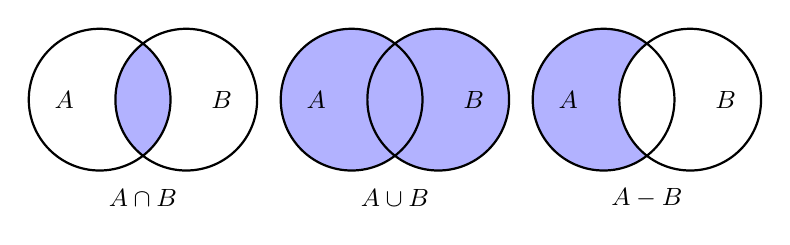
\begin{tikzpicture}[conjunto/.style={draw, thick}, font=\small]
    \def\r{0.9}                          % raio dos círculos
    % interseção: recorta pelo círculo A e pinta o círculo B
    \begin{scope}
      \clip (0,0) circle (\r);
      \fill[blue!30] (1.1,0) circle (\r);
    \end{scope}
    % união: pinta os dois círculos
    \fill[blue!30] (3.2,0) circle (\r) (4.3,0) circle (\r);
    % diferença: pinta A e "apaga" a parte de B, recortando pelo círculo A
    \fill[blue!30] (6.4,0) circle (\r);
    \begin{scope}
      \clip (6.4,0) circle (\r);
      \fill[white] (7.5,0) circle (\r);
    \end{scope}
    % contornos e rótulos
    \foreach \x/\op in {0/A \cap B, 3.2/A \cup B, 6.4/A - B} {
      \draw[conjunto] (\x,0) circle (\r) (\x+1.1,0) circle (\r);
      \node at (\x-0.45, 0) {$A$};
      \node at (\x+1.55, 0) {$B$};
      \node at (\x+0.55, -1.25) {$\op$};
    }
  \end{tikzpicture}
  \fonte{Elaborado pelo próprio autor.}
\end{figure}
%%END:venn

\end{document}
